\documentclass[a4paper,11pt]{jsarticle}


% 数式
\usepackage{amsmath,amsfonts}
\usepackage{bm}
% 画像
\usepackage[dvipdfmx]{graphicx}
\usepackage{here}

\usepackage[hang,small,bf]{caption}
\usepackage[subrefformat=parens]{subcaption}
\captionsetup{compatibility=false}


\begin{document}

\title{進捗報告}
\author{鷹見大地}
\date{\today}
\maketitle


\section{進捗}
複数パラメータを用いたCV-S法で複数の燃焼度における$k_{inf}$の不確かさを推定した。

\subsection{類似パラメータが2つの場合}
類似パラメータとして用いたのは、$5\mathrm{GWd/t}$のPu9の数密度および
$40\mathrm{GWd/t}$のPu2数密度を用いた。

結果を以下の図\ref{fig:1}に示す。

\begin{figure}[H]
  \begin{tabular}{cc}
    \begin{minipage}[t]{0.45\hsize}
      \centering
      \includegraphics[keepaspectratio,scale=0.5]{2}
      \subcaption{a1}
      \label{fig:1}
    \end{minipage} &
    \begin{minipage}[t]{0.45\hsize}
      \centering
      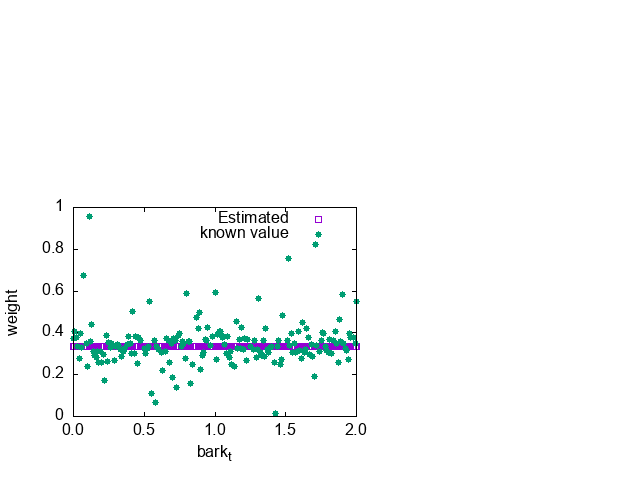
\includegraphics[keepaspectratio,scale=0.5]{weight2.eps}
      \subcaption{a2}
      \label{fig:2}
    \end{minipage} 
  \end{tabular}
  \caption{パターン1の結果}
  \label{fig:3}
\end{figure}


\end{document}